\begin{Exercise}[title={Stack},difficulty=5]
\label{ex:stack}
\Question \label{ex:stack q1} Create a simple stack which can hold a
fixed amount of \key{int}s. Is does not have to grow beyond this limit.
Define both a \func{push} and \func{pop} function.

\begin{wrapfigure}{l}{30mm}
\begin{center}
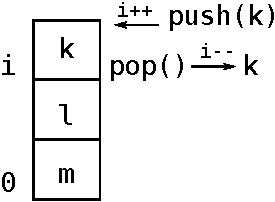
\includegraphics[scale=0.50]{fig/stack.pdf}
\end{center}
\end{wrapfigure}

\Question \label{ex:stack q2} Bonus. Write a \func{String} method which 
converts the stack to a string. This way you can print the stack using:
\lstinline{fmt.Printf("My stack %v\n", stack)}. This may aid in
debugging.
\end{Exercise}

\begin{Answer}

\Question 

\Question 

\end{Answer}
